\documentclass[colorful]{sty/itam-thesis}

\usepackage{lipsum}

\usepackage[
		showframe,
		paperwidth=17cm,
		paperheight=22.5cm,
		nofoot=true,
		bindingoffset=1.1cm,
		inner=1.6cm,
		outer=1.8cm,
		top=2.5cm,
		bottom=1.5cm
	]{geometry}

\usepackage{tikz}
\usepackage{tikzscale}
\usetikzlibrary{backgrounds, intersections, fillbetween}
% \usetikzlibrary{external}
% \tikzexternalize[prefix=tikz/]

\usepackage{import}

% Bibliografía
\usepackage{csquotes}
\usepackage[
	backend=biber,
    citestyle=alphabetic,
    style=alphabetic,
    maxcitenames=2,
    ]{biblatex}
\addbibresource{BachelorsThesis.bib}

% Paquete custom
\usepackage{sty/thesis-package}

\author{Alonso Martinez Cisneros}
\title{Approximate solutions to the Reinforcement Learning 
Problem via Linear Programming; with applications to Supervised 
Machine Learning.}
\date{2022}

\begin{document}

\frontmatter
\pagenumbering{roman}
\maketitle
\makefrontmatter

% Something
\cleardoublepage
% \pagestyle{plain}
% \pagenumbering{arabic}

\addcontentsline{toc}{chapter}{Dedication}

\vspace*{3cm}

\begin{center}
    A mi mamá y a mi papá. \\
    Porque mis logros son nuestros logros.
\end{center}

\medskip
\cleardoublepage
\addcontentsline{toc}{chapter}{Acknowledgements}
{
    \chapter*{Acknowledgments}

    Esta colección de hojas, letras e ideas representa la mayor cantidad de
    esfuerzo que he dedicado a una tarea específica en mi vida. Este trabajo y
    el esfuerzo que representa los dedico a mi familia y a mis amigos que son mi
    otra familia.

    Para Panini, Sofi Spinola, Juanito, Lothar, Ana Galán, Tonantzin, Rebe y Yonatan por compartir sus años itamitas conmigo, por obligarme a hacer tarea, y
    más de una vez preguntarse si ya había comido o tenía manera de llegar a
    casa.
    
    Para mi familia, que nunca ha dejado de poner su fé en mi. Para Sarah,
    Ankara, Max y Sandy por compartir la sobremesa conmigo.
    

    \bigskip

    Quiero agradecer a mi asesor Andreas Wachtel no solo por ser el buen asesor
    que fue, sino por haber servido como guía en el descubrimiento de las
    matemáticas que me apasionan a lo largo de mi carrera como estudiante en el
    \textsc{itam}. También agradezco a Arnaud Joly, parte del equipo de
    desarrollo principal de la librería scikit-learn por su guía sobre cómo
    implementar el algoritmo de árboles de clasificación y regresión, y al
    profesor Ashwin Rao de la universidad de Stanford por proveer sus notas del
    curso y responder un par de preguntas.
}
\addcontentsline{toc}{chapter}{Abstract}

\chapter*{Resumen}
En las últimas décadas avances en el campo conocido como Inteligencia Artificial
han cambiado el panorama de que problemas tienen y no tienen solución. Problemas
como procesamiento de lenguaje natural, reconocimiento de imágenes y otros,
ahora es posible resolver y son utilizados en nuestro día a día. Estos avances
se han dado gracias a la sinergia entre las Matemáticas y las Ciencias de la
Computación.

Estas herramientas pasaron de ser problemas abiertos en a investigación, a ser
problemas de ingeniería que se resuelven a escala día tras día. Una gran parte
de las personas involucradas en la implementación de estas soluciones tienen
conocimiento limitado sobre los conceptos matemáticos que subyacen la práctica
que llevan a cabo, lo cual es natural dado que no es conocimiento esencial para
sus tareas cotidianas. Esta tésis es un esfuerzo por explorar la teoría y las
intuiciones detrás de una de las técnicas más novedosas de la Inteligencia
Artificial: Aprendizaje por Refuerzo (\textsc{rl} por sus siglas en inglés).
Esta tesis busca sentar las bases en Procesos Estocásticos, Probabilidad, y
Optimización que dan el trasfondo para entender el aprendizaje por refuerzo. Se
busca presentar el contenido de manera intuitiva sin dejar de lado el rigor
matemático. Como matemático siento una obligación por presentar el campo de
estudio con la belleza que percibimos quienes lo estudiamos.

Esta tesis está compuesta por capítulos divididos en tres partes. La primera
parte presenta las ideas fundamentales de los diferentes campos de las
matemáticas que son esenciales para el aprendizaje por refuerzo, y una corta
introducción al campo del aprendizaje de máquina supervisado. La segunda parte
presenta en concreto lo que llamaremos el \emph{problema de aprendizaje por
refuerzo} en términos de un problema matemático, y desarrollamos la teoría que
permite dar soluciones aproximadas a este problema explicando porqué son de
interés. La tercera y última parte establece la conexión entre el aprendizaje de
máquina supervisado con el aprendizaje por refuerzo, y propone un algoritmo
basado en las soluciones aproximadas que son el foco principal de esta tésis al
problema de ajuste de árboles de decisión.

\chapter*{Abstract}
In the last 20 or so years, several advancements and novel techniques have
transformed the landscape of the discipline we currently call Artificial
Intelligence. These new approaches have made possible tasks deemed intractable
decades prior, such as natural language processing, image recognition, and
human-level competence at certain games, to name a few. These advancements have
come from a fruitful synergy between several fields of study: Mathematics and
Computer Science, to be precise.

As these techniques have moved from being the \textit{state of the art} to
mainly becoming a problem of engineering, most the people currently implementing
solutions based on Artificial Intelligence today have limited knowledge of the
mathematical underpinnings that enable such powerful methods, for they do not 
need it to do their job. This thesis represents an effort to explore the theory
and intuitions behind one of the most innovative techniques in Artificial
Intelligence: \acf{rl}. This work aims to explore the key ideas in
the areas of mathematics that provide the foundations for Reinforcement
Learning: Stochastic Processes, Probability Theory, and a particular emphasis on
Mathematical Optimization, so the field and problems can be presented in an
engaging fashion while sacrificing as little clarity as possible.

This thesis consists of mainly three parts, and several chapters that make up
said parts. The first part presents the main ideas from the different fields of
mathematics that will be needed to motivate and justify the theory behind
\ac{rl}, along with a brief introduction to the field of Supervised Machine
Learning. The second part develops the titular component of this thesis:
approximate solutions to the Reinforcement Learning Problem, motivating reasons
why approximations are desireable. Lastly, the third part motivates the framing
of an important problem in Supervised Machine Learning, the fitting of decission
trees, as a Reinforcement Learning Problem and proposes an algorithm based on
the approximate solutions developed earlier.
% %*******************************************************
% Abstract
%*******************************************************
%\renewcommand{\abstractname}{Abstract}
\addcontentsline{toc}{chapter}{Foreword}
\pdfbookmark[1]{Foreword}{Foreword}
% \addcontentsline{toc}{chapter}{\tocEntry{Abstract}}
\begingroup
\let\clearpage\relax
\let\cleardoublepage\relax
\let\cleardoublepage\relax

\chapter*{Foreword}
Brief, approachable statement of the objectives and scope of this thesis. To name a few of 
them:

\begin{itemize}
	\item Develop the theory in a leisurely style, sacrificing clarity as little as 
		possible.
	\item Contribute something to the field.
	\item Don't assume the reader to be a trained mathematician.
\end{itemize}

\endgroup

\vfill

% Foreword perhaps...

\tableofcontents

\mainmatter

%====================================================%
% Start of the content proper ---------------------- %
%====================================================%

% %===============================================%
% --- Dummy content for test-print purposes --- %
%===============================================%
\part{Primera parte}
\chapter{Hola}

\section{Sección Primera}
\lipsum[1-2]

\subsection{Subsección}
Un poco de matemáticas:

A \emph{policy} is a mapping from states to actions $\pi: S \to A$.

A \emph{value function} from a policy, written $V^{\pi}: S \to \R$ gives the expected sum 
of discounted rewards when acting under that policy
\begin{equation}
	V^{\pi} (s) = \E*{\sum_{t=0}^{\infty} \gamma^t R(s_t) \vertsep s_0 =s, a_t = \pi(s_t), 
	s_{t+1} \mid s_t a_t \sim P}
\end{equation}

Ahora referenciamos a \cite{ths:RodZ} para probar el hightlighting de cita. Ahora pruebo 
los theorem-like environments.

\begin{thrm}{Borel--Carathéodory}{borel-cara}
Let a function $f$ be analytic on a \emph{closed disc} of radius $R$ center origin.
Suppose that $r < R$. Then, we have the following inequality:
\begin{equation}
\|f\|_r \le \frac{2r}{R-r} \sup_{|z| \le R} \operatorname{Re} f(z) + \frac{R+r}{R-r} 
|f(0)|.
\end{equation}
\end{thrm}

Ahora, un corolario del teorema \ref{thm:borel-cara} bien inventado.

\begin{coro}{}{}
	Corolario sin título ni label.
\end{coro}

\subsubsection{Prueba de código}
Finalmente, un poco de código.

\begin{lstlisting}[language=julia, caption=Aplicando algoritmo de cifrado]
# Definiendo sistema de Lorenz
function lorenz!(du, u, p, t, σ=10, β=8//3, ρ=28)
    du[1] = σ * (u[2] - u[1])
    du[2] = u[1] * (ρ - u[3]) - u[2]
    du[3] = u[1] * u[2] - β * u[3]
end
\end{lstlisting}

Ahi va un lema:

\begin{lemma}{}{}
	Lemazo.
	\begin{equation}
		\E*{\sum_{k=0}^{\infty} \vertsep \Pe{A} }
	\end{equation}
\end{lemma}


\chapter*{Introduction}
% In the last 20 or so years a number of advancements and novel 
techniques have transformed the landscape of the discipline we 
currently call Artificial Intelligence. These new approaches have made 
possible tasks deemed intractable decades prior, such as natural 
language processing, image recognition and human-level 
competence at certain games, to name a few.  These advancements 
have come of a fruitful synergy between several fields of study: 
Mathematics and Computer Science to be precise.

As these techniques have moved from being the \textit{state of the 
art} to becoming mostly a problem of engineering, most of the people 
currently implementing solutions based on Artificial 
Intelligence today have a limited knowledge of the mathematical 
underpinnings that enable such powerful methods, for they do not 
need it to do their job.  This thesis represents an effort to 
explore the theory and intuitions behind one of the most 
innovative techniques in Artificial Intelligence: Reinforcement 
Learning.  The aim of this work is to explore the key ideas in 
the areas of mathematics that provide the foundations for 
Reinforcement Learning: Stochastic Processes, Probability 
Theory, and a special emphasis on Mathematical Optimization, so 
the field and problems can be presented in an engaging fashion 
while sacrificing as little clarity as possible.  Then, some 
selected problems and applications will be presented to 
illustrate the power of the techniques the reader has become 
acquainted to. 

As a mathematician I feel a special obligation to share the beauty of 
the ideas in our field to those outside of it. To that end and to make 
this work more enjoyable to the people I dedicate it to, I try to 
emulate a more leisurely style than the one found in research papers.  
Some terseness will be sacrificed in favor of clarity. Nevertheless, 
the mathematical minutia will not be ``swept under the rug'' or 
separated from the main body of text. Instead I will try to give 
context to the development of mathematical ideas, while not insisting 
on subjecting the reader to every single technical detail necessary 
for the formality of the arguments. The involved details will be 
available to those curious in appendixes.

This thesis consists of mainly three parts and several chapters that 
make up said parts. The first part presents the main ideas from the 
different fields of mathematics that will be needed to motivate and 
justify the theory behind Reinforcement Learning. The second part 
explores the Reinforcement Learning problems as the matter of 
Mathematics, and in particular how are these problems solved through 
different techniques in optimization. The third and final part deals 
with applications of Reinforcement Learning.

Interspersed among the purely mathematical theory are examples of how 
are these ideas expressed in the \href{https://julialang.org/}{Julia 
Programming Language}. These code snippets will be mostly self 
contained, ready to run, and leverage the vast ecosystem that makes 
Julia ideal for Mathematics and Scientific disciplines. Some code 
examples will play the role of pseudo code as Julia's simple syntax 
allows the mathematical ideas to shine through the implementation 
details.


\part{Foundations}

\chapter{Setting the stage}
% \section{A ``hand-wavy'' first approach}

What we refer to as Artificial Intelligence is a broad 
collection of methods and techniques used to solve a variety
of problems that we collectively associate with ``human 
intelligence'', such as identifying and classifying images, 
processing natural language, and learning from data.  Roughly 
speaking, the discipline can be divided into the following 
sub-fields of research:

\begin{itemize}
	\item Neural Networks.
	\item Computer vision.
	\item Natural Language Processing.
	\item Speech processing.
	\item Machine Learning.
\end{itemize}

This work is concerned specifically with Machine Learning.  
Particularly with a subset of the field known as Reinforcement 
Learning. Some authors such as \cite{sutton2020reinforcement} 
divide the field of Machine Learning (ML) in three parts: 
supervised learning, unsupervised learning, and reinforcement 
learning.  Both supervised and unsupervised learning rely 
heavily on statistics-based techniques such as regression 
models and statistical inference. The techniques used in 
reinforcement learning (RL), rely on different models of what 
learning is, and tries to go beyond finding association rules 
for a simple, well-defined problem.

In contrast to supervised learning where a learning agent is 
given data labeled by a knowledgeable source and must ``learn'' 
to classify based on those initial labels, in unsupervised 
learning as well as reinforcement learning, there is no 
``training data'', the agent must act and optimize its strategy 
based only upon the reward or penalty resulting from making a 
certain decision. The key words here are \textit{optimize}, 
\textit{strategy} and \textit{decision}.

For a concrete example picture an android at a casino playing 
at a slot machine, only this machine has $k$ levers instead of 
just one.  This robot is instructed to win as much money as 
possible across some number of games. How could this be 
achieved? Surely each lever makes the machine operate 
differently and thus is more or less likely to get a jackpot. 
If this android were a person, the approach would probably be 
to, across many games, try each lever and see how much money 
comes out. Hopefully, after the first few games this human 
player has a clear idea of which are the best levers to pull. 
This too might be a good strategy for the robot to employ, so 
lets explore that idea further.

If you think about it, the slot machine analogy is not so 
different from the standard mental model we have of say an 
infant learning to crawl.  With poor vision and only its 
caretaker's voice as guide, it must learn to find its way to 
safety by trial and error. It cannot be given millions of 
examples of ``valid paths'' for extrapolation, as is the case 
with supervised learning. This agent learns by interacting with 
the environment itself.

In a certain sense RL leverages our intuitions about the nature 
of learning. All the main elements are there: cause and effect, 
goals, and consequences to decisions made, but as we will see, 
it also encodes more subtle concepts. For instance, delayed 
gratification and planning ahead. It also has the novelty of 
being goal-oriented rather than task-oriented as most Machine 
Learning techniques often are. For example, a self-driving car, 
``trained'' via supervised learning might train on millions of 
examples on what constitutes a valid steering wheel move, is
expected to extrapolate to situations outside the training 
data. Meanwhile a self-driving car, learning by being evaluated 
is learning how to drive as an activity consisting of hundreds 
of little tasks, all to be mastered simultaneously.

\section{Formalizing ideas}
Now, mathematically speaking, what does it \textit{mean} for a 
machine to ``learn''?

We might not get as far as what learning as a whole means for 
humans or machines, but we can certainly discuss what 
mechanisms allow self-driving cars to exist or computers to 
beat world champions of Chess and Go. For that, we need to 
identify the key concepts in the picture I painted and express 
them in the language of mathematics.

For now, we can gloss over the details of how might a machine 
make decisions, perceive goals, take actions or perceive 
rewards. Let us focus on one key component: the ``learning''. 
When we talk about the process of a machine learning something 
we are thinking about something or someone (referred to as 
agent henceforth) that is able to keep track of the decisions 
it made before and whether or not they resulted in positive 
results so it can later on apply that knowledge to become an 
increasingly better problem solver. If this agent is evaluated 
each time it carries out some task, we would like for its score 
to increase each successive time it tries to complete the task. 
The idea of a continuously improving score is the foundation of 
mathematical optimization.

\subsection{Optimization Theory}
As the name suggests, mathematical optimization is concerned 
with finding an ``optimal'' (whatever ``optimal'' means) 
solution to problems where an unambiguous score might be given 
to different solutions. Even if there is no best solution to a 
given problem, the techniques used in mathematical optimization 
often allow for a continuous improvement through iteration.

Going back to our slot machine example, each time the robot 
selects one of the $k$ levers the machine gives out a prize. 
The prizes vary greatly in size, and there is no way to know 
which ones give the biggest prizes in advance. Since the robot 
wants to maximize money earned, if one lever is consistently 
giving out bigger prizes it is likely to keep pulling it. The 
robot was rewarded earlier for choosing that lever by getting a 
big prize.  Similarly if a lever pull resulted in no prize at 
all, the robot lost money by playing and probably will not 
choose that lever again. In each iteration the player robot 
would like to increase more and more the prize, and is thus  
encouraged to keep track of which levers give good prizes, 
improving the average prize in each successive game.

We are now ready to peel away another layer of abstraction.  We 
now have an intuition of what it means for a machine to learn, 
or in other words continually improve. But in the model we 
discussed earlier, the player is making choices along the way. 
A predefined path is not programmed or even known. If it were 
known this would not be a problem at all, the robot could 
choose the known-good levers every single time. Since that is 
not the case the robot must choose and balance between 
exploring and exploiting the knowledge gained so far. What does 
it mean for this robot player to ``make choices''?

\subsection{Stochasticity}
Another key aspect we take for granted when we talk about 
machines learning is implicit in the word learning. If there 
were a predefined path for the robot to take we would hardly 
call that learning, it is merely reproducing instructions.  
What this means for us, is that we must allow for a framework 
in which our robots actions are not completely determined 
beforehand. In fancier words, the succession of events that 
determine the robots actions and responses to stimuli are not 
predetermined or \textit{deterministic}.

This idea is formalized through something called a 
\textit{stochastic process}. The word stochastic is just 
mathematical lingo for ``not entirely determined beforehand'' 
or ``aptly described as a random phenomenon''.  In particular, 
we can think of the robot as being in some state among quite a 
few possible. The robot can change states as time goes by but 
the transitions are not always the same and they do not 
necessarily carry the same reward or punishment.

For instance, the robot at the slot machine might have gotten a 
very big prize the first time it chose a certain lever but got 
almost nothing the next game. The feedback it got by choosing 
an action changes as time goes by, because the slot machine 
behaves randomly. This robot had a certain amount of 
information after pulling the lever for the first time: this is 
a good lever to pull. In the next game this robot already knows 
which lever might be a good bet, so among the $k$ possible 
options it might choose to pull the same lever as last time. 
Next time the reward is much smaller, the robot transitioned 
states in a sense. It was in a state were the best option was 
somewhat clear, to a state in which that one lever is no longer 
the most desirable option. It went from being certain to being 
forced to explore. We might think of this process a navigating 
the branches of a tree, making a decision every time a branch 
forks of into smaller branches.

[AQUI DIAGRAMA DE ARBOL]

\section{A slightly more nuanced example}
One of the major achievements and claims to fame for 
reinforcement learning in the past decades has been its use in 
some of the most famous matches in several classic board games.  
Chess was ``mastered'' when Kasparov, then chess grandmaster, 
was beaten by Deep Blue in 1997 \cite{silver2018chess}. Other 
board games with enormous state spaces such as Go, the game 
that originated in China, proved to be too complex for the 
techniques used by Deep Blue. Deep Blue was mainly based on 
hard-coded openings and endgames taken from other grandmaster 
games, which differs a lot from the RL approach. Go was much 
later attacked by another robot player named AlphaGo, developed 
by researchers from a company named DeepMind 
\cite{silver2017mastering}.  AlphaGo defeated Lee Sedol, the 
reigning human champion in 2016.  AlphaGo was one of the most 
notorious applications of RL and made the field even more 
popular. Since RL has proved to be very good for these kinds of 
tasks in the past, let us explore an example with a simpler 
board game.

\subsection{Duopoly, oligopoly, \ldots}
Consider a simplified version of a popular game whose name I 
avoid using as it might be copyrighted. This game consists of a 
circuit with predefined squares, some available for sale, in 
which a player is at any given moment. In order to move, a 
player spins an arrow fixed on the center of a circle that can 
stop at any of four circle segments numbered from 1 to 4. This 
is the number of squares the player moves forward. We refer to 
this spinning arrow as the \textit{spinner}.

You can find a scaled version of this game's board in figure 
\ref{fig:miniopoly-board}. The squares numbered 1 through 8 
(colored in shades of red, blue, purple and green) are 
available for purchase, while the white squares indicate a 
special action such as allowing the player to spin once more in 
the same turn, complete the circuit by going directly to the 
starting square and so on.

Going forward, picture a robot being ``trained'' to become a 
super player via the RL techniques we are slowly developing. At 
each turn the robot spins and moves forward however many 
squares the spinner indicates. If the robot lands on any square 
with a number on it, it might acquire that square for itself. 
From that moment on, if the opponent lands on that square the 
robot player will be paid rent. If the robot lands on that same 
square, it may build hotels on it so next time the opponent 
lands there, the rent payed will be much higher. The robot also 
receives money every time it completes the circuit.

As you might have guessed, the point of the game is to make the 
most amount of money. The game ends when either the robot or 
it's opponent go bankrupt. What purchase strategy must the 
robot follow to win?
\begin{figure}[H]
	\centering
	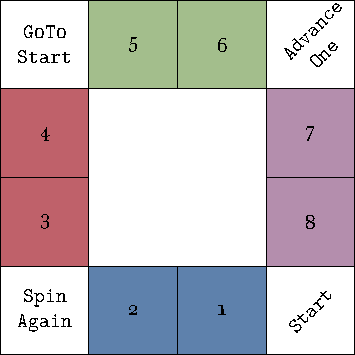
\includegraphics[width=.65\textwidth]{img/board.pdf}
	\caption{Board for the game described earlier.}
	\label{fig:miniopoly-board}
\end{figure}

First off, unlike the slot machine-playing robot, this robot 
player cannot entirely choose which square to move to, it can 
only decide if it wants to purchase it or not once it has 
landed on it. The biggest number it can spin is 4, and even if 
it got to spin again the furthest it could go is square 5. Even 
if the robot wanted to go to square number 8 and buy it, there 
is no possible way to do that.

Figure \ref{fig:miniopoly-diagram-start} shows a simplified 
version of the board. Only the squares accessible on the first 
turn are shown, along with arrows indicating the possible 
transitions between the starting square and the rest.
\begin{figure}[h]
	\centering
	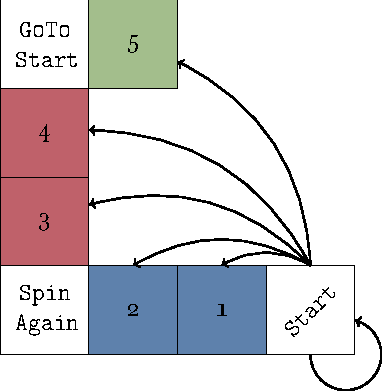
\includegraphics[width=.65\textwidth]{img/diagram-start.pdf}
	\caption{Squares accessible on the first turn.}
	\label{fig:miniopoly-diagram-start}
\end{figure}

In figure \ref{fig:miniopoly-diagram-start} we can see all the 
possible squares the robot might land on and then buy starting 
from the first turn. Notice how squares 6 and further are not 
included. If the robot were to spin a 4, the red square with 
number 3 is the furthest it could go. If it were to land on 
\texttt{Spin Again} and then spin a 4, the largest possible 
spin, it could move four squares: from \texttt{Spin Again} to 
3, then to 4, then to \texttt{Goto Start}, and finally to 
square 5, exhausting its possible moves.

Notice how in this figure we only care about the starting and 
ending points, not the transit points, so that is why there are 
no arrows pointing to the squares that move the player 
elsewhere like \texttt{Spin Again} and \texttt{Goto Start}. 
This is the reason there is an arrow that points from 
\texttt{Start} to itself. This transition might happen. In 
fact, we know what it takes for this to happen: land on 
\texttt{Spin Again}, and then land on \texttt{Goto Start}. In 
other words, this transition happens if the robot spins a 3 two 
consecutive times.

If the robot were to land on \texttt{Spin Again}, then spin a 
3, it would ``land'' on \texttt{Goto Start}, finishing its turn 
back at the starting square. That particular move results in 
the robot going back to the start and getting paid for 
completing the circuit, without running the risk of landing on 
a square someone else owns. That sounds like a very desirable 
move (for us looking at the big picture, the robot cannot see 
that far ahead yet). Since we would like this to happen, we 
might ask how likely is for that to happen.

\begin{figure}[h]
	\centering
	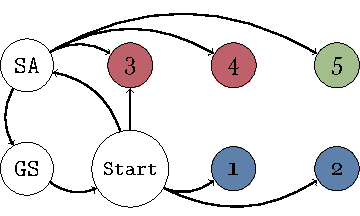
\includegraphics[width=\textwidth]{img/transicion.pdf}
	\caption{Diagram showing the possible transitions to the 
	numbered squares, starting the turn at \texttt{Start}. 
	Squares \texttt{GoTo Start} and \texttt{Spin Again} are 
	abbreviated as \texttt{GS} and \texttt{SA} respectively.}
	\label{fig:miniopoly-transicion}
\end{figure}

Lets try to analyze how likely the robot is to end up in this 
particularly rewarding situation. For that it's often helpful 
to think of the possible steps that lead to it. On figure 
\ref{fig:miniopoly-transicion} we can see a more abstract 
diagram of the possible movements the robot might make, and 
this time we are taking into account intermediate squares. Each 
arrow represents where the robot might land after spinning, not 
necessarily it's final resting square. Now, using some very 
basic probability theory we can calculate how likely it is for 
the robot to ``take that route'' so to speak. Once we do, we 
can calculate how likely a ``route'' or sequence of arrows is.

\begin{figure}[h]
	\centering
	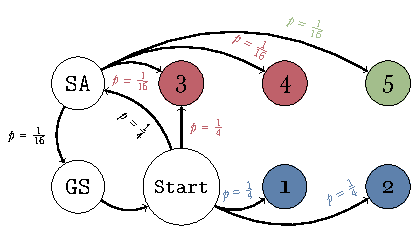
\includegraphics[width=\textwidth]{img/transicion-markov.pdf}
	\caption{Transition diagram with transition probabilities}
	\label{fig:miniopoly-transicion-markov}
\end{figure}

At the moment it is not important why some arrows have certain 
probabilities, and some might not be terribly obvious even for 
someone acquainted with some basic probability. In figure 
\ref{fig:miniopoly-transicion-markov} to find the probability 
of getting to a certain square (say 6 for example) we look only 
at the last arrow, as it takes into account the probability of 
the previous step happening. For example, the probability of 
the move that takes the player from \texttt{Start} back to 
\texttt{Start} we can look at the bottom left corner of figure 
\ref{fig:miniopoly-transicion-markov}. The player moves to 
\texttt{Spin Again} with probability 1/4 because the spinner 
has an equal chance of making the player move either 1, 2, 3 or 
4 squares. Once the player is on \texttt{Spin Again} and spins 
once more, it has a chance of 1/16 of landing on \texttt{GoTo 
Start}. The final arrow pointing from \texttt{GoTo Start} to 
\texttt{Start} is not annotated with the probability of it 
happening, since that transition is not random. Once the player 
lands there, the next thing that happens to the player is 
always the same: go to the starting square.

The robot we are trying to teach moves as the figure above 
suggests. There is a different diagram for each square in which 
the player finds itself at the start of its turn. The robot is 
not aware of this, all it knows is that it spins, and then is 
transported elsewhere and must decide whether to buy or not (if 
the square is available). All it knows is it's current 
position, and the gains or losses it sustained on the other 
squares it has visited. Crucially, landing on a square 
previously visited does not necessarily mean the reward will be 
the same as last time. For instance, if it lands on square 3 
and decides not to buy it, the reward was a net 0, but the 
other player may buy it so that the next time the robot visits 
that square it has to pay rent, which would mean a loss. Also, 
the reward for buying a square may come much later on or not at 
all. This robot must somehow keep track of what the expected 
reward for landing somewhere might be, recording it somewhere 
and tallying up as it goes.

For instance after a few turns it might have something fig. 
\ref{fig:hist-miniopoly} on its head to help make decisions.

After playing a few games, keeping a record of which squares it 
bought, the player might make a graph to discover what moves it 
made that resulted in higher rewards at the end of the game. 
Such a graph might look like figure \ref{fig:hist-miniopoly}, 
which is a violin plot. In this plot, a violin-shaped figure 
gives the robot an idea of what squares yielded better rewards 
or smaller losses when bought or when left for other players to 
buy. The height of the violin indicates how high the reward was 
at the end of the game, while the width of the violin helps the 
robot decide whether that outcome was a fluke or not. A thin 
violin at a specific height (reward) indicates that over the 
games it has played so far, that specific reward marked by the 
y-axis is not as common as the reward that corresponds to the 
thicker parts of the violin.
% Se entiende??

\begin{figure}
\centering
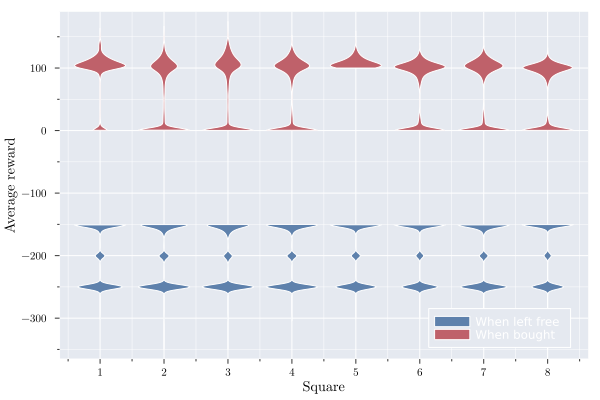
\includegraphics[width=\textwidth]{img/hist-miniopoly.tikz}
\label{fig:hist-miniopoly}
\caption{Violinplot}
\end{figure}

This figure was created by simulating N-THOUSAND games and 
recording what rewards the robot player obtained at the end of 
the game by buying or not buying a certain square. For 
instance, if it bought square 3, the record shows the initial 
loss of however much money the player paid for the square. 
Later on in the game if the opponent lands on square 3 and pays 
rent, that rent is recorded as a gain for the robot player. 
That number is averaged out at the end of the game so the robot 
can analyze this information later. One way of analyzing this 
information to improve strategy is precisely to make a graph 
like the one in figure \ref{fig:hist-miniopoly}

Its stands to reason that as this graph is updated the learning 
agent will be able to make progressively better choices by 
identifying the patterns. For instance, it might notice from 
figure \ref{fig:hist-miniopoly} that buying SQUARE ALGO 
consistently results in higher rewards at the end of the game. 
The robot noticed this because the violin corresponding to 
SQUARE ALGO is noticeably higher than the others. Simple as 
this example might be, the essence is similar to the powerful 
programs that defeat world champions of chess and Go.

This example covers most of the core ideas of what is referred 
to as the Reinforcement Learning Problem. We will explore the 
ideas presented here in much more detail along this thesis and 
crucially, focus on something we left out on this example. How 
can a purchase strategy be improved upon?

\section{Wrapping up}
So far we have developed a mental model of what to do should we 
wish to teach a robot how to drive or beat a world champion of 
Go. The rest of this thesis is dedicated to the careful 
development of the ideas here presented into the language of 
mathematics. Specifically, tackling questions such as:
\begin{itemize}
	\item What mechanism allows the robot player to learn from 
	experience and fine-tune it's strategy to become better?
	\item How can we tell when a new strategy is better than an 
	old one?
	\item Is it possible to find \textit{the} best strategy? 
	How difficult is it?
\end{itemize}

Beyond mere description, this exercise has the potential to 
unlock \textit{insight}. As is often said by legendary math 
communicator Grant Sanderson\footnote{From the YouTube channel 
\href{https://www.youtube.com/channel/UCYO_jab_esuFRV4b17AJtAw}{3blue1brown}}(loose 
quote), the point in formulating things this way is to gain a 
deeper understanding of the phenomenon. So let's dive right in.


\chapter{Probability Theory}

\chapter{Stochastic Processes \& Markov Decision Processes}
% 
\label{chapter:Stochastic}

To be filled\ldots



\begin{dfn}{Stochastic Process}{stochastic-process}
\end{dfn}

\begin{dfn}{Markov's Property}
    Given a stochastic process made up of random states $S_t$ for times $t = 0,
    1, 2, \dots$, we say it satisfies the \emph{Markov property} (or is
    \emph{Markovian}) if the probalities of transition between $S_t$ and
    $S_{t+1}$ satisfy
    \begin{equation*}
        \P \left[ S_{t+1} \mid S_t, S_{t-1}, \dots, S_0 \right] = \P \left[ S_{t+1} \mid S_t \right],
    \end{equation*}
    for all $t \geq 0$.
\end{dfn}

Markov's property is often called the ``memoryless property'', since in essence,
it says the history of the process does not influence the future evolution, it
is only determined by the present state.

\begin{dfn}{Markov Decision Process}{MDP}
\end{dfn}

\chapter{Optimization Theory}

\chapter{Reinforcement Learning}
% 
\label{chapter:ReinforcementLearning}

On Chapter~\ref{chapter:motivation} we presented a very simple 
example of a problem that may be solved via Reinforcement 
Learning: a robot trying to play a game we called Miniopoly. As 
simple as that example was, the key ideas will now allow us to 
delve into the theory proper, and formalize some ideas while 
hopefully giving satisfying answers to some questions that the 
intuitive treatment might have left open.

\section{The Agent \& the Environment}
Recall from Chapter~\ref{chapter:Motivation} that we referred 
to the robot player as a ``learning agent''. This agent is 
continuously interacting with the rest of the game and 
surveying its current state. As we saw earlier, the robot then 
selects an action on the basis of this current game state.

To be precise, say that the game starts at some $t=0$ and ends 
at $t=T$. We discretize this period of time into $t \in \{0, 1, 
2, \ldots \}$ At each of these points $t$ in time, the agent 
finds itself at some state $S_t \in \States$, where $\States$ 
represents the set of all possible states. This defines exactly 
what we called a stochastic process back in 
Chapter~\ref{chapter:Stochastic}: a series of random variables 
$\{ S_t \}_{t = 0, 1 \ldots}$. 

Likewise, at each time step $t$ the agent chooses how to 
interact with an action $A_t \in \Actions(s)$, where 
$\Actions(s)$ is the set of all \textit{available} actions at 
the current state $s$. This too forms a stochastic process. One 
time step in the future $t+1$ the agent receives more feedback 
from the environment, the so-called reward signal $R_{t+1} \in 
\Rewards \subseteq \R$. This process moves forward from $t$ to 
$t+1$ and so on until the task is over. This defines a Markov 
Decision Process (MDP from now on), which we can reorder as 
follows:
\begin{equation}
	S_0, A_0, R_1, A_1, R_2, S_2, A_2, R_3, \ldots
\end{equation}

This particular ordering makes it easy to see why we chose to 
discretize time into steps. This illustrates how at each time 
step the agent surveys the state, and based on it selects a 
\textit{feasible} action. The next time step begins when the 
robot receives a reward signal from the environment. 

A key idea is subtly hidden in the notation. Notice how only 
the set of actions depends on a particular $s$. Both the set of 
states $\States$ and the set of rewards $\Rewards$ are in a 
certain sense independent of $s$. Why is it that only 
$\Actions(s)$ is dependent on $s$?

The ``Markov'' in Markov Decision Process is exactly what makes 
the set of actions special. As covered in 
Chapter~\ref{chapter:Stochastic}, a Markov process is often 
used to describe stochastic transitions between a set 
of---emphasis on terminology here---\textit{states}. In the 
example on Chapter~\ref{chapter:Motivation} the states were the 
literal squares in the game. And as we discussed, not every 
state is accessible from any other state. Thus, it makes sense 
that for each state the set of possible actions is determined 
by it. Some transitions are just impossible.

Not only are some transitions impossible at certain states, a 
given action chosen by the agent will not always result in the 
same transition from the state $s$ to the state $s'$, which 
might sound obvious as we have already established that this 
entire process can be best modeled by a MDP. To study the 
probability of a certain transition from state $s$ to state 
$s'$ given that a certain action $a \in \Actions(s)$ was taken 
we introduce the \textit{dynamics} function, keeping with the 
notation in \cite{SuttonBarto}.

\begin{dfn}{Dynamics function}{dynamics-func}
	For all $s, s' \in \States, r \in \Rewards, a \in 
	\Actions(s)$, we define the \emph{dynamics function} $f: 
	\States \times \Rewards \times \States \times \Actions(s) 
	\to [0, 1]$ as follows:
	\begin{equation*}
		p(s', r \mid s, a) \coloneqq \IP{S_t = s', R_t = r 
		\vertsep S_{t-1} = s, A_{t-1} = a}.
	\end{equation*}
\end{dfn}

Hola \ref{dfn:dynamics-func}


% FIXME: ESTO NO TIENE CONTEXTO, PONERLO
\begin{equation}
	\label{eq:prop-dependencia-vq}
	v_* (s) = \max_{a \in \Actions} q_* (s, a) \quad \forall \s in \States.
\end{equation}

\part{Approximate solutions to the Reinforcement Learning 
Problem}

\chapter{Approximate Linear Programming}
\chapter{Approximate Linear Programming}
\label{chapter:ApproximateLinearP}
\section{Introduction}

As discussed in previous chapters \ref{chapter:ReinforcementLearning}, the
problem of finding the best policies by using Bellman's optimality equations
falls within the realm of dynamic programming. The problem is that even if an
explicit solution can be given under certain conditions, the computational
burden of calculating exact solutions is often too significant to overcome, even
on modern computing equipment. And given the ``curse of dimensionality'', even
if the contemporary problems became tractable in the future thanks to the
ever-increasing computing power, that very same improvement in computing power
would motivate researchers to tackle bigger still problems. So, to use the
\ac{rl} techniques, we must find a way to use our computational resources more
efficiently. 

Since Reinforcement Learning happens to be part of the techniques often grouped
under the umbrella of ``artificial intelligence'', it has enjoyed much attention
for decades. Thanks to these research efforts and numerous applications in the
industry, there are several battle-tested approximate solutions to the \ac{rl}
problem we have developed here. Among these are: Q-learning, Monte--Carlo
estimation methods, temporal difference learning, and many others that are
described in detail in \cite[Chapter~4]{SuttonBarto}. The somewhat novel
technique described in this thesis was developed in the first decade of the
2000s and is not part of the standard toolbox for solving \ac{rl} problems since
it was developed initially in the area of management science and particularly
for the problem of probabilistic inventory management, following previous work,
laid out since the 1960s. 

Specifically, the technique to be laid out in this part of the thesis was
developed by \citeauthor*{farias2003LP2ADP}, as a continuation of previous work
by \citeauthor*{denardo1970} and \citeauthor*{depenoux1963} in
\cite{denardo1970} and \cite{depenoux1963}, respectively. In a nutshell,
\citeauthor*{farias2002thesis} casts the dynamic programming problem that arises
from solving Bellman's optimality equations as a linear program and then gets
around the curse of dimensionality by using linear approximations for the
interest functions to reduce the number of variables in the problem. Without
further ado, let us get to the details right after developing the necessary
background.

\section{Exact Dynamic Programming}

In Chapter \ref{chapter:ReinforcementLearning}, we showed that using Bellman's
optimality equations, we can obtain optimal policies if we have access to the
optimal value ($v_*$) or action-value ($q_{*}$) functions. We denote these
functions subindexed by $*$ to accentuate the fact that they are optimal in the
sense that they satisfy Bellman's optimality equations, which are
\eqref{eq:bellmans-value} and \eqref{eq:bellmans-action-value} for $v_*$ and
$q_*$ respectively. 
\begin{align}
v_{*}(s) &= \max_{a} \sum_{s', r} p(s', r \mid s, a) \left[ r + \gamma v_{*} (s')
\right], \label{eq:bellmans-value} \\
q_{*}(s, a) &= \sum_{s', r} p(s', r \mid s, a) \left[ r + \gamma \max_{a'} q_{*}
(s', a') \right], \label{eq:bellmans-action-value}
\end{align}
for all $s \in \States, a \in \Actions$.

Equation \eqref{eq:bellmans-value} is important, but not that helpful in
practice. It tells us the best possible reward a learning agent can expect in a
learning task. In other words, the best possible reward \textit{after} the agent
followed the best policy but tells us very little about how to obtain that
policy. We would like to predict the total reward a given policy will yield.
Thankfully, in chapter \ref{chapter:ReinforcementLearning}, we obtained an
expression to calculate the expected reward a given policy $\pi$ will yield
starting from a certain state $s$, that we will refer to as \textit{Bellman's
recurrence equation} from now on: 
\begin{equation}
\label{eq:bellmans-recurrence}
% TODO: Transcribir (4.4) de S&B.
v_\pi (s) = \sum_{a \in \Actions} \pi(a \mid s) \sum_{s', r} p(s', r \mid s, a) \left[ r + \gamma v_{\pi}(s') \right].
\end{equation}

The identity \eqref{eq:bellmans-recurrence} was proved earlier in chapter
\ref{chapter:ReinforcementLearning} in Lemma \ref{lem:recursive-eval}, the
Recursive Evaluation Lemma. We named the Lemma that way for reasons that will
become apparent soon.

Using \eqref{eq:bellmans-recurrence} we can obtain an exact solution for $v_\pi$
solving one equation for each state $s \in \States$. This is often called the
\textit{prediction problem} in the literature \cite[Chapter~4.1]{SuttonBarto}.
Transforming equation \eqref{eq:bellmans-recurrence} we obtain the following,
simpler expression:
\begin{align}
\label{eq:bellmans-recurrence-prime}
v_\pi(s) &= \sum_{a} \pi(a \mid s) \sum_{s', r} p(s', r \mid s, a) \left[ r + \gamma v_\pi (s') \right] \nonumber \\
&= \sum_{a} \pi(a \mid s) \left[ \sum_{s', r} r p(s', r \mid s, a) + \gamma \sum_{s', r} v_\pi (s') p(s', r \mid s,a) \right] \nonumber \\
&= \sum_a \pi(a \mid s) \underbrace{\sum_{r} r \sum_{s'} p(s', r \mid s, a)}_{r(s,a) \text{(by dfn. \ref{dfn:rewards-func})}} +
    \gamma \sum_{a} \pi(a \mid s) \sum_{s', r} v_\pi (s') p(s', r \mid s, a) \nonumber \\
&= \sum_{a} \pi(a \mid s) \left[ r(s,a) + \gamma \sum_{s'} p(s' \mid s, a) v_\pi (s') \right] \tag{\ref*{eq:bellmans-recurrence}$\prime$}.
\end{align}

Since \eqref{eq:bellmans-recurrence-prime} defines one equation for each state,
we can think of the system of linear equations defined in terms of vectors and
matrices. This approach will later serve to define Bellman's policy\footnote{or
``one-step'' \cite[pg.~9]{nadeemward2021}, or ``expectation backup''
\cite[Lect.~3, Contraction Mapping]{silver2015}, the literature uses various
names. We follow \cite{raoRL4F}.} and optimality operators, a powerful tool.

For now, let us consider the value function as a vector, following
\cite[pg.~132]{raoRL4F}. Specifically,
\[
    \vec{v} = \left[ v (s_1), \dots , v (s_{|\States|}) \right].
\]
As shorthand notation we define $\vec{v}(s) \coloneqq v(s)$. Recall that $r(s,
a)$ is the expected reward upon taking action $a$ being in state $s$, and $p(s'
\mid s, a)$ is the probability of transitioning directly from state $s$ to state
$s'$ after taking action $a$. We define:
\begin{align*}
    R_\pi (s) &= \sum_{a \in \Actions} \pi(a \mid s) \, r(s,a), \\
    P_\pi (s, s') &= \sum_{a \in \Actions} \pi(a \mid s) \sum_{s' \in \States} p(s' \mid s, a),
\end{align*}
which result from a slightly rearranged version of
\eqref{eq:bellmans-recurrence-prime}.

We denote by $\vec{R}_\pi$ the vector $\left[ R_\pi(s_1), \dots, R_\pi
(s_{|\States|}) \right]$ and $\vec{P}_\pi$ the stochastic matrix $\left[
P_\pi(s_i, s_j) \right]$ that defines the transition probabilities from any
state $s_i$ to every other distinct state $s_j$ with $i, j \in \left\{ 1, \dots,
|\States| \right\}$. As promised, this is the key to what will become one of our
most powerful tools: Bellman's policy operator.  This will enable us to study
how \textit{any} $v$ acts on the set of states $\States$.

\begin{dfn}{Bellman's Policy Operator}{bellmans-pol-operator}
    We denote by $T_\pi$ the operator $T_\pi: \R^{|\States|} \to \R^{|\States|}$
    defined as:
    \[
        T_\pi \vec{v} = \vec{R}_\pi + \gamma \vec{P}_\pi \vec{v},
    \]
    for any value function vector $\vec{v} \in \R^{|\States|}$. The definition
    of this operator can be found in \cite[Ch.~5.4]{raoRL4F}.
\end{dfn}

Using the newly defined Bellman's Policy Operator, we can rewrite Bellman's
recurrence equation \eqref{eq:bellmans-recurrence} as
\begin{equation}
    \label{eq:BPO-fixed-point}
    T_\pi \vec{v}_\pi = \vec{v}_\pi.
\end{equation}
This means $\vec{v}_\pi$ is a fixed point of the Bellman Policy Operator.

Using the same arguments that led to \eqref{eq:bellmans-recurrence-prime}, let
us write Bellman's optimality equation for the value function
\eqref{eq:bellmans-value} using another operator.

\begin{dfn}{Bellman's Optimality Operator}{bellmans-opt-operator}
    We denote by $T_*: \R^{|\States|} \to \R^{|\States|}$ \emph{Bellman's Optimality Operator}, defined for each $s \in \States$ as:
    % FIXME: Aqui change r(s,a) va multiplicado con vector de 1's.
    \[
        (T_{*} \vec{v})(s) = \max_{a \in \Actions} \left\{ r(s, a) + \gamma \sum_{s' \in \States} p(s' \mid s, a) v(s') \right\}. 
    \]
\end{dfn}

Using the Optimality Operator, \eqref{eq:bellmans-value} can be rewritten as
\begin{equation}
    \label{eq:bellmans-optimality-operators}
    T_* \vec{v}_{*} = \vec{v}_{*}.
\end{equation}

% In other words, the optimality operator $T_*$ is a non-linear operator with a
% fixed point $\vec{v}_*$ \cite[Ch.~5.4]{raoRL4F}.

Theorem \ref{thrm:farias2002thesis-thrm2.1} (corresponding to Theorem 2.1 in
\cite[Ch.~2.2]{farias2002thesis}) presents some key properties of Bellman's
Policy Operator. We are especially interested in the fact that it has a unique
fixed-point.

\begin{thrm}{}{farias2002thesis-thrm2.1}
    Let $\vec{v}$ be an arbitrary value function. Then,
    \begin{enumerate}
        \item $\left\| T\vec{v} - T \vec{v}_* \right\|_{\infty} \leq \gamma
            \left\| \vec{v} - \vec{v}_* \right\|$.
        \item If $\vec{v}_0 \geq \vec{v}_1$, then $T\vec{v}_0 \geq T\vec{v}_1$.
        \item The operator $T$ has a unique fixed-point given by $\vec{v}_*$.
    \end{enumerate}
\end{thrm}

The equation presented in \eqref{eq:BPO-fixed-point} is equivalent to statement
3 on the previous theorem. As promised, Bellman's operators yield the solutions
to both the prediction problem and the optimal value function, which come in
handy to prove whether or not our \ac{rl} problem has solutions or under which
circumstances. However, so far, we have no idea how to solve them.

With our toolbox almost complete, it is time to advance our search for
optimality. As previously mentioned, there are several approaches to solving
Bellman's equations (\eqref{eq:bellmans-value} and
\eqref{eq:bellmans-action-value}) are based on dynamic programming, yielding
several algorithms we do not review in detail in this thesis as they are outside
of scope. The literature for those techniques is excellent. If interested in a
more detailed treatment of said algorithms, please review \cite{SuttonBarto} and
\cite{raoRL4F}.

\subsection{Approaching optimality}

So far, our goal has been to find the ``best'' policy, but what does it mean for
a policy to be the best? We can not compare policies directly, but we can
compare the value function's value for each of them. The optimal, the
``best'' policy is the one that maximizes the value function.

\begin{dfn}{Optimal Policy}{optimal-policy}
    We say that a given policy $\pi$ is in a certain sense \textit{better} than
    the policy $\pi'$, which we write as $\pi \geq \pi'$, whenever $v_\pi(s)
    \geq v_{\pi'} (s)$ for every $s \in \States$. This is called a partial
    ordering over the space of policies. A policy $\pi_*$ is optimal if
    $\pi_*(s) \geq \pi (s)$ for all $s$ and all other policies $\pi$.
\end{dfn}

The equality in definition \ref{dfn:optimal-policy} is only satisfied when both
policies are optimal, as stated in the following Lemma which correspondes to
Lemma 4.10.2 in \cite[pg.~115]{raoRL4F}.

\begin{lemma}{}{equality-on-optimality}
    For any two optimal policies $\pi^{*}_{1}$ and $\pi^{*}_{2}$, for all $s \in
    \States$ they evaluate to the same on the value function, that is,
    $v_{\pi^{*}_{1}} (s) = v_{\pi^{*}_{2}} (s)$.  Using the vector notation
    introduced earlier, $\vec{v}_{\pi_{1}^{*}} = \vec{v}_{\pi_{2}^{*}}$.
\end{lemma}

\begin{proof}
    Since $\pi_{1}^{*}$ is an optimal policy, from the optimal policy definition
    we have: $v_{\pi_{1}^{*}}(s) \geq v_{\pi_{2}^{*}} (s)$ for all $s$.
    Likewise, since $\pi_{2}^{*}$ is also an optimal policy, $v_{\pi_{2}^{*}}(s)
    \geq v_{\pi_{1}^{*}} (s)$ for all $s$. Therefore, $v_{\pi_{1}^{*}}(s) =
    v_{\pi_{2}^{*}} (s)$ for all $s$.
\end{proof}

Wielding Lemma \ref{lem:equality-on-optimality} we can prove that there always
exists an optimal policy for the \ac{rl} problem we have been studying.

\begin{thrm}{}{opt-policy-existence}
    For a Reinforcement Problem based on a discrete-time, finite-space Markov
    Decision Process, the following hold:
    \begin{itemize}
        \item There exists an optimal policy $\pi_*$. That is, $v_{\pi_*} (s)
            \geq v_{\pi}(s)$ for all other policies $\pi$ and all states $s \in
            \States$.
        \item All optimal policies achieve the optimal value function given by
            \eqref{eq:bellmans-value}. That is, $v_{\pi_*}(s) = v_* (s)$ for all
            $s \in \States$ where $\pi_*$ is one optimal policy.
        \item All optimal policies achieve the optimal action-value function,
            given by \eqref{eq:bellmans-action-value}.
    \end{itemize}
\end{thrm}

\begin{proof}
    We follow the proof in \cite[pg.~115]{raoRL4F} closely.

    As a consequence of Lemma \ref{lem:equality-on-optimality}, we only need to
    find a policy that maximizes both the value and action value functions,
    achieving the maximum values: $v_*$ and $q_*$ respectively.

    A policy that is a candidate to be optimal can be constructed as follows:
    \begin{equation}
        \label{eq:greedy-policy-construction}
        \pi_{*}^{D} (s) = \argmax_{a} q_{*} (s, a) \quad \forall s \in \States.
    \end{equation}

    For now, we assume that the resulting action $a$ for any given state $s$ is
    unique.

    We show that $\pi_{*}^{D}$ maximizes the optimal value and action-value
    functions. As established in chapter \ref{chapter:ReinforcementLearning},
    equation \eqref{eq:prop-dependencia-vq}, $v_* (s) = \max_a q_* (s, a)$, and
    therefore,
    \[
        v_* (s) = q_* \left(s, \pi_{*}^{D}(s) \right).
    \]

    In other words, we maximize the value function if we first take the action
    prescribed by the policy $\pi_{*}^{D}$ followed by the action from the next
    time steps that maximize the value function, and so on. This is precisely
    why Bellman's recurrence equations work as they do. Likewise, since the
    state-value and action-value can be expressed in terms of each other as
    reviewed in chapter \ref{chapter:ReinforcementLearning} the action-value
    function is maximized following whatever action $\pi_{*}^{D}$ prescribes.
    Formally,
    \[
        q_{\pi_{*}^{D}} (s, a) = q_* (s,a) \quad \forall s \in \States, a \in \Actions.
    \]

    Lastly, we show that $\pi_{*}^{D}$ is an optimal policy by contradiction.

    Suppose that $\pi_{*}^{D}$ is not an optimal policy. That means that there
    exists some other policy $\pi$ such that $\pi > \pi_{*}^{D}$. In the partial
    order defined previously, that means that $v_{\pi} (s) > v_{\pi_{*}^{D}}
    (s)$ for at least one state $s$! This contradicts the definition of the
    optimal value function $v_* (s) = \max_\pi v_\pi (s)$ for all $s$. Therefore
    $\pi_{*}^{D}$ must be an optimal policy.
\end{proof}

Notice how the optimal policy was constructed by prescribing to the state $s$
whichever action maximizes the value function at that state. In other words, the
policy constructed was \emph{greedy}. A much more exciting and aesthetically
pleasing way of proving theorem \ref{thrm:opt-policy-existence} is by using the
properties of Bellman's operators. Theorem 5.4.1 in \cite[pg.~130]{raoRL4F},
reproduced below, allows us to conclude similar things to Theorem
\ref{thrm:opt-policy-existence}.

\begin{thrm}{Policy Evaluation Convergence Theorem}{pect}
    The value function $\vec{v}_\pi$ is the \underline{unique} fixed-point of
    the Bellman Policy Operator $T_\pi$, and
    \[
        \lim_{t \to \infty} (T_\pi)^{i} \vec{v}_0  \to \vec{v}_\pi,
    \]
    for any starting $\vec{v}_0$.
\end{thrm}

The proof of Theorem \ref{thrm:pect} can be found in \cite[pg.~131]{raoRL4F}. We
do not include the proof it it requieres a considerable amount of preliminaries
and is extensive. Nonetheless, we think it is a very pleasing application of
Banach's Fixed-Point Theorem.

Theorem \ref{thrm:opt-policy-existence} guarantees the existence of an optimal
policy in theory. But we are interested in finding such a policy in practice,
preferably in a way that is computable this century. Luckily, Theorem
\ref{thrm:pect} provides an update rule that converges to the stationary point
of Bellman's Policy Operator and thus the optimal value function. That approach
is called \emph{value iteration} and is described in detail in
\cite{SuttonBarto,raoRL4F}, we focus on other approaches.

\section{Approximate Linear Programming}

Having established the necessary context, we can at last address the main
objective of this Chapter, and indeed the whole thesis: avoiding the use of
inefficient dynamic programming and use linear programming (LP) to solve
Bellman's equations. We reproduce Theorem 6.2.2 in
\cite[Ch.~6.9.1]{puterman2014}, adapted to our notation, as this is the basis
for the LP formulation.

\begin{thrm}{}{6.2.2-puterman}
    Suppose there exists a value function $\vec{v}$ for which
    \begin{enumerate}
        \item $\vec{v} \geq T_{*} \vec{v}$, then $\vec{v} \geq \vec{v}_*$.
        \item $\vec{v} \leq T_{*} \vec{v}$, then $\vec{v} \leq \vec{v}_*$.
    \end{enumerate}
\end{thrm}

By Theorem \ref{thrm:6.2.2-puterman}, statement 2, whenever a given policy
$\vec{v}$ satisfies
\[
    \vec{v} \leq T_* \vec{v}
\]
which then, by Bellman's optimality equation
\eqref{eq:bellmans-optimality-operators} gives
\[
    \vec{v} \leq \vec{v}_* = T_* \vec{v}_*,
\]
where vectors $\vec{v}$ and $\vec{v}_*$ are compared component-wise. In other
words, we can try to find a lower bound $\vec{v} \leq T_{*} \vec{v}$ by
considering Definition \ref{dfn:bellmans-opt-operator} which gives the following
set of linear constraints:
\[
    v(s) \leq \max_{a} \left\{ r(s, a) + \gamma \sum_{s'} p(s' \mid s, a) \, v(s') \right\} \quad \forall s \in \States.
\]
In particular
\begin{equation}
    \label{eq:upper-bound-v}
    v(s) \leq r(s, a) + \gamma \sum_{s'} p(s' \mid s, a) \, v(s') \quad \forall s \in \States, a \in \Actions.
\end{equation}

Since the solution to \eqref{eq:bellmans-optimality-operators} is guaranteed to
exist by Theorem \ref{thrm:opt-policy-existence} and satisfy: $\vec{v}_* = T_*
\vec{v}_*$, we can approach it by finding the biggest vector upper bound. We
can generate lower bounds to the optimal value function by using
\eqref{eq:upper-bound-v}.

Finding the biggest upper bound leads to the following optimization problem:
\begin{equation}
\begin{array}{rl@{}ll}
    \displaystyle \max_{v: \States \to \R} & v(s) \\
    \text{Subject to} & \displaystyle v(s) \leq r(s,a) + \gamma \sum_{s'} p(s' \mid s, a) \, v(s') & \quad \forall a \in \Actions, s \in \States. \\
    & v(s) \text{ unconstrained,} & \quad \forall s \in \States.
\end{array}
\end{equation}

Utilizing the vector notation introduced earlier, we can find a Linear Program formulation to the previous optimization problem
\begin{equation}
\label{lp:exact-lp}
\tag{ELP}
\begin{array}{rl@{}ll}
    \displaystyle \max_{\vec{v} \in \R^{|\States|}} & \vec{c}^{\top} \vec{v} \\
    \text{Subject to} & \vec{v} \leq \vec{R}_a + \gamma \vec{P}_a \, \vec{v} & \quad \forall a \in \Actions \\
    & \vec{v} \text{ unconstrained.} &
\end{array}
\end{equation}
With $\vec{R}_a \in \R^{|\States|}$ defined as $[r(s_1, a), r(s_2, a), \dots,
r(s_{|\States|}, a)]^{\top}$ and $\vec{P}_{i,j}^{a} = p(s_j \mid s_i, a)$.

Professor \citeauthor{farias2002thesis} refers to Linear Program
\eqref{lp:exact-lp} as the \textit{exact Linear Program}
\cite[Ch.~2.3]{farias2002thesis}. This LP (linear program) has $|\States|$
variables and $|\States| \times |\Actions|$ constraints. This makes it
tremendously vulnerable to the curse of dimensionality, since we have as many
variables to optimize as states. Solving this LP for the number of states in a
modern \ac{rl} problem becomes prohibitively computationally expensive, even
when the average-case complexity of solving an LP is polynomial
\cite[pg.~147]{kochenderfer2022}, much better than listing the $|\States|!$
states.

To overcome this prohibitive cost, we turn to one of math's most proliferous
ideas: linear approximations. By approximating the function $v$ with a linear
basis we hope to reduce the number of variables, but the number of constraints
will remain the same. Chapter \ref{chapter:PropertiesGuarantees} proposes a way
to reduce the number of constraints.

\subsection{Linear everything}

Approximating complicated functions by collections of linear or linear-affine
functions is not new. One of the most proliferous applications of this idea is
linear regression in the area of statistical learning, or its more glamorous
name: machine learning. The main idea behind linear regression is approximating
a relationship between a vector of \textit{regressors}, $\vec{x}_i$, measured
attributes observed for some phenomenon of interest; and a vector of response
variables $\vec{y}$. Specifically, the relationship to be estimated is the
conditional expectation of $\vec{y}$ given the $\vec{x}_i$, or $\mathbb{E}
\left[ \vec{y} \mid \vec{x}_i \right]$. In a nutshell, the relationship is
modeled by a linear function $\vec{x}_{i}^{\top} \vec{B}$. The matrix $\vec{B}$
is filled with coefficients that minimize the distance between the approximation
and the actual observed values $\vec{x}_i$. The key idea is that these
parameters are obtained by measuring the error between the predicted linear
relationship and the true, observed values. The exact nature of this process is
not important at the moment, but it is important to keep in mind that it can
only be carried out if we have access to the actual observed values of interest
$(\vec{x}_i, y_i)$. For our problem of interest, we have no such luxury. We have
to be a bit more clever.

\subsubsection{Linear architecture}
The strategy followed in \cite{farias2002thesis} is generating scoring functions
with a pa\-ra\-me\-trized class of functions, similar to linear regression but
carrying out the ``fitting'' without being able to sample the function we are
trying to approximate.

This parametrized class of functions will be a basis for the space of value
functions made up of linear functions $\varphi_i : \States \to \R$ for $i = 1,
\dots, K$, with $K \ll |\States|$ a set parameter. Following the standard
notation used in statistics, we denote $\widehat{\vec{v}} \approx \vec{v}$ the
linear approximation to the value function.

\begin{dfn}{Basis matrix}{}
    We define a matrix $\Phi \in \R^{|\States| \times K}$ given by:
    \[
        \Phi =
        \begin{bmatrix}
            | & \vdots & | \\
            \varphi_1 & \cdots & \varphi_K \\
            | & \vdots & |
        \end{bmatrix}.
    \]
\end{dfn}

This way, use the representation for $\widehat{\vec{v}} = \Phi \vec{\beta}$,
where $\vec{\beta}$ is a vector of parameters that will fit this representation.
Armed with this one last tool, let us take another look at the exact LP
\eqref{lp:exact-lp}, substituting the function for the approximation wherever
pertinent:
\begin{equation}
\label{lp:approx-lp}
\tag{ALP}
\begin{array}{rl@{}ll}
    \displaystyle \max_{\vec{\beta} \in \R^{K}} & \vec{c}^{\top} \Phi \vec{\beta} \\
    \text{S.t.} & \displaystyle \Phi \vec{\beta} \leq \vec{R}_a + \gamma \vec{P}_a \, \Phi \vec{\beta} & \quad \forall a \in \Actions, \\
    & \vec{\beta} \text{ unconstrained}.
\end{array}
\end{equation}

Once having an approximately optimal value function we can generate optimal
decisions according to:
\begin{equation}
    u_{\Phi \beta} (s) = \argmin_{a} \left( \vec{R}_a + \gamma \vec{P}_a \Phi \beta \right),
\end{equation}
where the policy $\pi$ is subscripted by $\Phi\beta$ to emphasize how it is
generated.

The LP in \eqref{lp:approx-lp} is referred to as the \textit{approximate linear
program}. The vector $\vec{c}$ with positive components is called the
\emph{state-relevance weights} vector and determines, in a sense, the role each
basis function plays in approximating a certain characteristic of the target
function. Notice that the number of variables in this LP reduced from
$|\States|$ to $K$. The number of constraints was not reduced, but according to
\cite{farias2002thesis}, most of them become inactive, and solutions can be
approximated efficiently with modern methods. The rest of
\citeauthor{farias2002thesis}'s work shows how the special structure inherited
from dynamic programming can be used to efficiently sample constraints, making
the solution of this LP more efficient.

The subsequent chapters of this part are dedicated to briefly reviewing the
extensions and results of this method.  Chapter
\ref{chapter:PropertiesGuarantees} continues the exploration of the Approximate
Linear Programming (ALP) method we have just described. In particular, some
desirable properties the optimization problem \eqref{lp:approx-lp} has and some
performance guarantees we can expect.


\section{Bibliographic Notes}

For the development of Bellman's Optimality Operator, we follow several sources:
\begin{itemize}
    \item Bellman's original paper \cite{bellman1957}.
    \item Several lectures and corresponding notes:
    \begin{itemize}
        \item David Silver's Course \cite[Lects.~2-3]{silver2015}.
        \item Basic Reinforcement Learning course at McGill University
            \cite[Lect.~2]{moisescu-parejaa}.
        \item Foundations of Reinforcement Learning with Applications in Finance
            course textbook by Ashwin Rao \cite[Ch.1-4]{raoRL4F}.
    \end{itemize}
    \item \citeauthor{nadeemward2021}'s thesis \cite{nadeemward2021} which
        summarizes the numerical approaches based on dynamic programming skipped
        in this chapter.
    \end{itemize}

For a more thorough development of why Bellman's Operator is defined, please
consult any of the sources referenced directly above.

The conceptual leap involved in casting the dynamic programming problem as a
linear program using the properties of Bellman's operators, entire chapters are
dedicated to explaining the background and motivating the ideas, and laying a
solid foundation in \cite{puterman2014}, specifically chapters 2 and 6.

Sadly, we are constrained in scope and can not possibly lay the entire
groundwork for this idea to feel more natural and better motivated. For the
interested reader, \citeauthor{puterman2014}'s book is a great, if involved,
read and is cited by several other bibliographic pieces used in this chapter.

%% Aqui todos los resultados de Farias que menciona LPinRL.

\part{Applications to Supervised Machine Learning}

\appendix

\chapter{Simulating Miniopoly}
\chapter{Simulating Miniopoly}
\label{appendix:MiniopolySim}

\section*{Code used to simulate the game described on earlier 
chapters.}

The specific rules for the game described in chapter 
\ref{chapter:Motivation} can be best visualized as literal 
code. Listing \ref{lst:main-logic} contains the actual code 
used to check and enforce buying and renting rules, as well as 
carry out transactions. All code presented here is valid Julia 
code.

\lstinputlisting[language=julia, firstline=161, lastline=200, 
caption=Main logic for the game, 
label={lst:main-logic}]{../codigo/simulacion-miniopoly/Miniopoly.jl}

The code above depends on the definition of several ``Objects'' 
in Object Oriented Programming parlance: 
\lstinline{GameManager}, \lstinline{Player} and 
\lstinline{Square}.

The \lstinline{Player} Structure represents a single player of the game. The
code in listing \ref{lst:player-def} shows what attributes or fields
characterize it (i.e. the information we keep track of). Notice for instance the
attribute \lstinline{rewardslog}, which is a mapping between a 
\lstinline{Square} represented as its number and its ownership status to a
number. This is the mechanism that keeps track of the reward obtained by buying
or not a certain square.

\lstinputlisting[language=julia, firstline=6, lastline=10, 
caption=Definition of Player structure, 
label={lst:player-def}]{../codigo/simulacion-miniopoly/MiniopolyPieces.jl}

The \lstinline{Square} Structure represents a purchasable 
square as defined by the game rules outlined on chapter 
\ref{chapter:Motivation}. 

\lstinputlisting[language=julia, firstline=53, lastline=56, caption=Definition of Square structure, label={lst:square-def}]{../codigo/simulacion-miniopoly/MiniopolyPieces.jl}

The \lstinline{GameManager} Structure is essentially what keeps 
track of the property ledger, the current state of the game, 
among other things. Listing \ref{lst:gamemanager-def} shows 
what information is kept for book-keeping purposes.

\lstinputlisting[language=julia, firstline=57, lastline=62, 
caption=Definition of GameManager structure, 
label={lst:gamemanager-def}]{../codigo/simulacion-miniopoly/Miniopoly.jl}

The results of this simulation are presented in chapter
\ref{chapter:Motivation}.

\nocite{*}
\printbibliography

\end{document}